\documentclass[crop=false]{standalone}
\usepackage[utf8]{inputenc}
\usepackage{amsmath}
\usepackage[dvipsnames]{xcolor}
\usepackage{pdfpages}
\usepackage{enumerate}
\usepackage{amssymb}
\usepackage[framemethod=default]{mdframed}
\usepackage[nomarginpar,left=2cm,right=2cm,top = 2cm, bottom = 2cm]{geometry}

\renewcommand{\thesubsection}{\thesection.\alph{subsection}}
\renewcommand{\thesubsubsection}{\thesection.\alph{subsection}.\roman{subsubsection}}

\mdfdefinestyle{theoremstyle}{%
linecolor=black,linewidth=.3pt,%
frametitlerule=true,%
frametitlebackgroundcolor=blue!5,
innertopmargin=\topskip,nobreak=true,
}

\mdfdefinestyle{theoremstyle_break}{%
linecolor=black,linewidth=.3pt,%
frametitlerule=true,%
frametitlebackgroundcolor=blue!5,
innertopmargin=\topskip,nobreak=false,
}

\mdfdefinestyle{style2}{frametitle={},%
             linewidth=.3pt,topline=true,backgroundcolor=blue!3!green!8!}

\mdtheorem[style=theoremstyle]{task}{Angabe}
\mdtheorem[style=theoremstylebreak]{taskbreak}{Angabe}

\newmdenv[style = style2,title=false]{solution}

\begin{document}
\begin{taskbreak}[Liapunovstabilität und Linearisierung]
 Betrachten Sie das System
\[
\left[\begin{array}{c}{\dot{x}_{1}} \\ {\dot{x}_{2}}\end{array}\right]=\left[\begin{array}{c}{x_{1} x_{2}-2 x_{1}^{2}} \\ {-5 x_{1}^{2}+2 x_{1}-x_{2}+2 x_{1} x_{2}}\end{array}\right]
\]
mit der Ruhelage $x_{s}=0 .$ Mit der Liapunovfunktion
\[
V\left(x_{1}, x_{2}\right)=\frac{5}{2} x_{1}^{2}-2 x_{1} x_{2}+\frac{1}{2} x_{2}^{2}
\]
erhält man
\[
\dot{V}\left(x_{1}, x_{2}\right)=-4 x_{1}^{2}+4 x_{1} x_{2}-x_{2}^{2}
\]
\begin{enumerate}[i]
    \item Welche Stabilitätsaussage können Sie für die Ruhelage $\mathbf{x}_{s}=\mathbf{0}$ anhand des um
die Ruhelage linearisierten Systems treffen? Begrüindung!
    \begin{solution}
    Berechnung der linearisierten $\mathbf{A}$-Matrix:
    \[\mathbf{A} = \frac{\partial\mathbf{f}\left( \mathbf{x}_s \right)}{\partial\mathbf{x}}
    =\begin{pmatrix}
    0 & 0\\
    2 & -1
    \end{pmatrix}\]
    Die Eigenwerte dieser Matrix:
    \[ \text{det}\left( \mathbf{A} - \mathbf{E}\lambda \right) = -\lambda \left(-1-\lambda\right) = \lambda^2 + \lambda=0 \rightarrow \lambda_1 = 0, \quad \lambda_2 = -1\]
    Alle Eigenwerte liegen in der linken Halbebene, jedoch existiert ein Eigenwert mit Realanteil = 0, damit lässt sich laut Satz 7.4 aus dem Übungsskriptum keine Aussage über die Stabilität des nichtlinearen Systems treffen.
    \end{solution}
    \item Welche Stabilitätsaussage können Sie für die Ruhelage $\mathbf{x}_{s}=0$ machen, wenn Sie
nur die Funktionen $V$ und $\dot{V}$ betrachten? \emph{Begründung! HINWEIS: Sie können
davon ausgehen, dass $V\left(x_{1}, x_{2}\right)$ positiv definit ist.}
\begin{solution}
Es muss die Definitheit von $\dot{V}$ bestimmt werden:
\[0 \geq - \underbrace{\left( -2x_1 + x_2 \right)^2}_{\text{immer $\geq 0$}} = -\left(4x_{1}^2 - 4 x_1 x_2 + x_2^2 \right) = \dot{V} \]
$\dot{V}$ kann als binomischer Term mit negativen Vorzeichen geschrieben werden. $\dot{V}$ ist also negativ semidefinit. Hiermit kann gezeigt werden, dass die betrachtete Ruhelage stabil ist, über die asymptotische Stabilität kann keine Aussage gemacht werden.
    \end{solution}
    \item Bestimmen Sie die Menge $S=\left\{\left(x_{1}, x_{2}\right) \in \mathbb{R}^{2} | \dot{V}\left(x_{1}, x_{2}\right)=0\right\}$ und skizzieren Sie
diese in der $\left(x_{1}, x_{2}\right)$ -Ebene.
\begin{solution}
Aus der vorherigen Zeile kann erkannt werden das $S$ die Menge an Tupeln ist, welche die Gleichung
\[-2 x_1 + x_2 = 0\]
erfüllt. In der $x_1$-$x_2$-Ebene ist das offensichtlich eine Linie durch den Ursprung.
    \end{solution}
    \item Zeigen oder widerlegen Sie unter Zuhilfenahme Ihrer Skizze, dass die größte gegenüber dem Fluss des Systems (1) positiv invariante Menge in $S$ die Ruhelage $\mathbf{x}_{s}=\mathbf{0}$ ist.
    \begin{solution}
    Wenn man die Trajektorien und die Invariante Menge S in einer gemeinsamen Skizze zeichnet erkennt man, dass nur die stationäre Trajektorie $\mathbf{x_s}=\mathbf{0}$ vollständig in dieser Menge enthalten ist:
    {\centering
        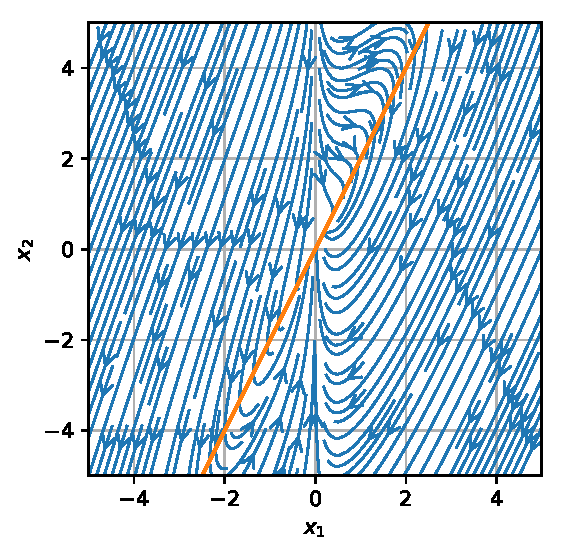
\includegraphics[width = 8cm]{LaSalle2016.pdf}
        \par}
        In der Menge $S$ gilt: $x_2 = 2 x_1$, wenn man diesen Zusammenhang in die Systemgleichung einsetzt erhält man folgendes (entspricht dem Tangentialvektor der Trajektorien an der orangen Linie):
        \[
\left[\begin{array}{c}{\dot{x}_{1}} \\ {\dot{x}_{2}}\end{array}\right]=\left[\begin{array}{c}{0} \\ {-x_1^2}\end{array}\right]
\]
Wie in der Skizze schon zu erahnen bestätigt sich hier, dass alle von $\mathbf{0}$ verschiedenen Trajektorien die Menge $S$ immer von "oben nach unten" schneiden und nicht in der Menge bleiben.
    \end{solution}
    
\item Welche Aussage können Sie mit dem Ergebnis von Punkt (iv) über die Stabilität
der Ruhelage $\mathbf{x}_{s}=\mathbf{0}$ machen?
\begin{solution}
 Mit dem Invarianzprinzip von LaSalle konnte die asymptotische Stabilität der Ruhelage gezeigt werden. \end{solution}
\end{enumerate}
\end{taskbreak}
\end{document}